%%%%%%%%% JPS abstract %%%%%%%%%%%%%%%%%%%%%%%%%%%%%%%%%%%%%%%%%%
\documentclass[12pt,a4paper,upLaTeX]{jsarticle}

%%%%%%%%% packages %%%%%%%%%%%%%%%%%%%%%%%%%%%%%%%%%%%%%%%%%%%%%%
\usepackage[dvipdfmx]{graphicx} % Include figure files
\usepackage[%                           % 余白の設定
%mag=1400,%                              jarticle の場合（14ptに）
dvipdfm,truedimen,%
top=30truemm,bottom=50truemm,%
left=20truemm,right=20truemm]{geometry}
\usepackage{fancyhdr}
\usepackage{amsmath,amssymb}
\usepackage{bm}
\pagestyle{fancy}

%%%%%%%%% header %%%%%%%%%%%%%%%%%%%%%%%%%%%%%%%%%%%%%%%%%%%%%%%%
\begin{document}

\fancyhf{}
\setlength{\headheight}{60pt}   % ある程度大きめに
\fancyhead[R]{大阪大学大学院 理学研究科 物理学専攻 博士前期課程2年\\
学籍番号 24B25011\\
加島 駿一\\}

\setlength{\footskip}{20pt}
% \fancyhf{}
\fancyfoot[C]{集中講義 素核実験におけるデータ収集 レポート}

\fancyfoot[R]{\thepage}

\vspace{50pt}
\begin{center}
{\gt \Large 学んだこと・それを活かして今後やりたい調査 }\\[14pt]

\end{center}

\vspace{10pt}
%%%%%%%%%%%%%%%%%%%%%%%%%%%%%%%%%%%%%%%%%%%%%%%%%%

\subsubsection*{学んだこと・興味を持ったこと}
\begin{itemize}
  \item Extended デッドタイムとNon extended デッドタイムの違い
  \begin{itemize}
    \item 言葉通り、デッドタイム中に新たな入力があったらデッドタイムが伸びるか否か
    \item DAQの観点で言うと、デッドタイムの間の信号を受け付けるかどうか
    \item ライブタイム率の計算式が変わる
    \begin{itemize}
      \item Extended デッドタイムの場合:
      \begin{align}
        L_{ratio} = e^{-R\tau}
      \end{align}
      \item Non-Extended デッドタイムの場合:
      \begin{align}
        L_{ratio} = \frac{1}{1+R\tau}
      \end{align}
    \end{itemize}
    \item しかしながら解析的に解けるのはイベントがランダムに発生する事象(ポアソン分布)に限られる
  \end{itemize}
  \item イベントのランダム性がない場合のデッドタイムに興味を持ち、自分の研究で使っているデータ収集システムにおけるデッドタイムを知りたいと感じた。
\end{itemize}
\subsubsection*{気になって調べた(調べてみたい)こと}
私の研究テーマはJ-PARCのMARQ実験で使われる連続読み出し式DAQに実装するオンラインフィルターの開発と評価である。以下の項目を研究のスコープに含めている。
\begin{itemize}
  \item 目的: 不要なデータを削減すること(どうやって削減するかも含めて)と、それをオンラインで実現するために必要な計算資源の量の調査
  \item 連続読み出ししたデータの中でどのようにイベントパケットを定義するか
  \item イベントパケットごとに詳細な解析をしてデータの取捨選択をどのように行うか
  \item 必要な処理ごとに要求される計算資源の量の見積もり
  \begin{itemize}
    \item (必要に応じて)解析アルゴリズムの改善
  \end{itemize}
\end{itemize}
上記のうちイベントパケットをどのように切り出すかについては、関心のある物理事象を捉えるために最小限の速いカウンターのコインシデンスを基準にしたウィンドウを用いることになっている。その後に切り出したウィンドウを解析して、例えば散乱粒子の有無によってイベントパケットを取捨選択する。ここで問題になりうるのがイベントのオーバーラップである。オーバーラップしたイベントでは解析効率(関心があるイベントを関心のあるイベントだと判断できた数/関心のあるイベントの数)が低下すると考えられる。最も保守的な見積もりだと、イベントのオーバーラップが起きると解析ができなくなると仮定するだろう。このとき、解析効率にExtended デッドタイムの考えが適用できると考えた。もしイベントの発生がランダムであれば解析効率を計算することができるが、図\ref{fig:beam_structure}に示すような時間的な構造を持ったビームでどれくらいの解析効率になるか気になったので今後調査を行うつもりである。

\begin{figure}[tbhp]
  \centering
  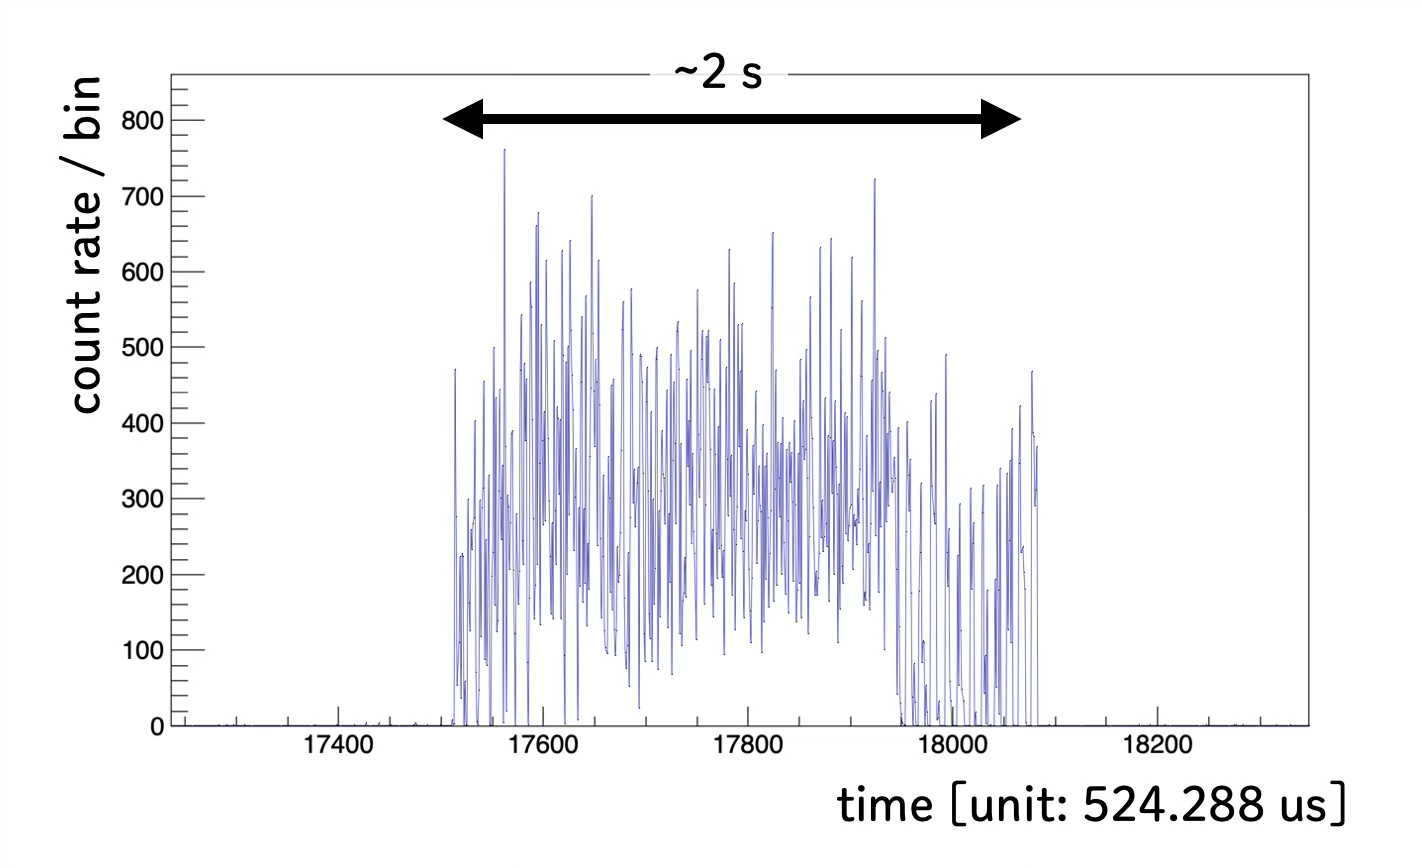
\includegraphics[width=0.8\textwidth]{./PICTURE/beam_structure.png}
  \caption{J-PARC ハドロン実験施設に供給されるビームの時間的な構造の例。約2秒の間、加速器施設のメインリングから徐々にビームを取り出すSlow extractionと呼ばれる方式でビームを検出器に照射している。横軸は時間で、縦軸は検出器のカウントレートである。}
  \label{fig:beam_structure}
\end{figure}

% J-PARCにあるハドロン実験施設に供給されるSlow extractionビームを用いる


\end{document}